\documentclass[a4paper,12pt,oneside,final]{article}
\usepackage[left=15mm,top=15mm,right=15mm,bottom=20mm]{geometry}
\usepackage{tikz}
\usepackage{float}
\usetikzlibrary{arrows,positioning,shapes.geometric}

\title{%
Redes Neuronales \\
MNIST Auto-Encoder \\*[23pt]
Trabajo Práctico 3 \\
}
\date{2020}
\author{Igor Andruskiewitsch}

\begin{document}
    \maketitle

\section{Introducción}

En este trabajo vamos a implementar un auto-encoder para el dataset MNIST utilizando la librería PyTorch. Un auto-encoder es una herramienta utilizada en el área de computer vision, cuyo objetivo es comprimir y descomprimir una imágen. Un ejemplo de aplicación ampliamente usada de auto-encoders es la de modelos de segmentación, que identifican (usando una clasificación por pixel) los objetos de una imágen.

\section{Modelo}

Existen distintas formas de implementar un auto-encoder, una forma ampliamente utilizada son las redes convolucionales. Sin embargo, en este caso, al contar con imágenes significativamente pequeñas (el MNIST cuenta con imágenes de $28 \times 28$) vamos utilizar una red neuronal simple. La arquitectura de nuestra red neuronal va a ser la siguiente:

\begin{figure}[htp]
\centering
\tikzset{%
  every neuron/.style={
    circle,
    draw,
    minimum size=1cm
  },
  neuron missing/.style={
    draw=none, 
    scale=4,
    text height=0.333cm,
    execute at begin node=\color{black}$\vdots$
  },
}

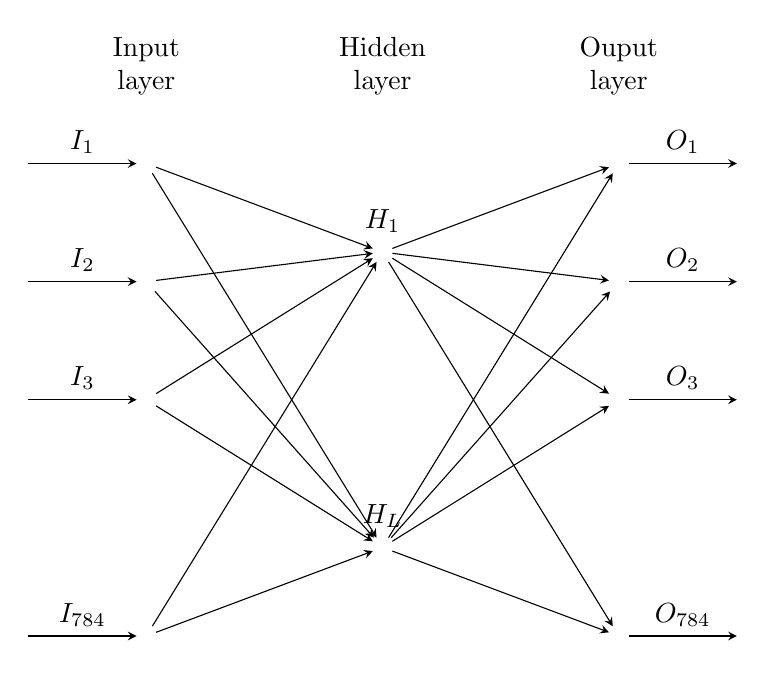
\begin{tikzpicture}[x=1.5cm, y=1.5cm, >=stealth]

\foreach \m/\l [count=\y] in {1,2,3,missing,4}
  \node [every neuron/.try, neuron \m/.try] (input-\m) at (0,2.5-\y) {};

\foreach \m [count=\y] in {1,missing,2}
  \node [every neuron/.try, neuron \m/.try ] (hidden-\m) at (2,2-\y*1.25) {};

\foreach \m [count=\y] in {1,2,3,missing,4}
  \node [every neuron/.try, neuron \m/.try ] (output-\m) at (4,2.5-\y) {};

\foreach \l [count=\i] in {1,2,3,784}
  \draw [<-] (input-\i) -- ++(-1,0)
    node [above, midway] {$I_{\l}$};

\foreach \l [count=\i] in {1,L}
  \node [above] at (hidden-\i.north) {$H_\l$};

\foreach \l [count=\i] in {1,2,3,784}
  \draw [->] (output-\i) -- ++(1,0)
    node [above, midway] {$O_{\l}$};

\foreach \i in {1,...,4}
  \foreach \j in {1,...,2}
    \draw [->] (input-\i) -- (hidden-\j);

\foreach \i in {1,...,2}
  \foreach \j in {1,...,4}
    \draw [->] (hidden-\i) -- (output-\j);

\foreach \l [count=\x from 0] in {Input, Hidden, Ouput}
  \node [align=center, above] at (\x*2,2) {\l \\ layer};

\end{tikzpicture}
\caption{Arquitectura NN para nuestro auto-encoder.}\label{fig:nn}
\end{figure}

Observamos en la figura \ref{fig:nn} que la cantidad de inputs/outputs que tenemos es de $784$ ya que, como mencionamos anteriormente, las imágenes del MNIST son de $28 \times 28$. Un dato para agregar respecto a la arquitectura que vamos a usar es que vamos a introducir una no-linearidad $ReLU$ para la capa de {\bf input} y la {\bf hidden layer}. Por otro lado, para la capa de {\bf output} vamos a introducir la función de activación $Sigmoide$, ya que sabemos que las imágenes del MNIST están en escala de grises y los valores de sus pixeles se limitan al rango $(0, 1)$.

Vemos que para la capa oculta no definimos una cantidad fija de neuronas, si no que la denotamos con la letra $L$. Esto es porque a lo largo del trabajo vamos a variar este valor para observar cómo cambia la performance de nuestro modelo. También, luego de la activación $ReLU$ de la capa de {\bf input}, introducimos un Dropout con probabilidad $0.1$ para evitar que nuestro modelo se sobreajuste (overfit), es decir que aprenda a la perfección los datos de entrenamiento y no generalice.

\section{Entrenamiento}

En esta sección vamos a mostrar los resultados de entrenar nuestro modelo con $L = 64$. Utilizamos la función de pérdida {\it MSE} ({\it i.e.} Mean Square Error) y el optimizador {\it SGD} ({\it i.e.} Stochastic Gradient Descent). El entrenamiento se realizó por $50$ épocas, con un {\it learning rate} de $e^{-3}$, un {\it weight decay} de $e^{-5}$ y un {\it batch size} de $1000$.

Para poder medir la performance de nuestro modelo a través de las épocas, además del valor de la pérdida, vamos a utilizar la {\it Binary Accuracy}. Esta métrica consiste en redondear los valores de los pixeles de ambas imágenes (la original y la reconstruida por la red) y calcular el promedio de valores acertados por la red. El redondeo se realiza ya que como mencionamos anteriormente, las imágenes están en escala de grises y necesitamos tomar valores concretos para compararlas. Esta métrica, a diferencia de la {\it pérdida}, no va a afectar a los parámetros de nuestro modelo.

Para visualizar la performance del modelo a través de las épocas de entramiento, vamos a graficar los valores de la pérdida y la accuracy en conjunto:

\begin{figure}[ht]
  \centering
  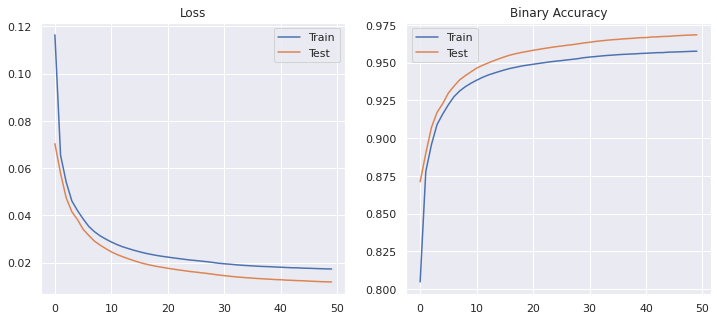
\includegraphics[width=15cm,keepaspectratio]{./graficos/training_metrics.png}
  \caption{Pérdida y Accuracy para $L=64$}\label{training_metrics}
\end{figure}

En estos gráficos observamos que tanto para la pérdida como para la accuracy, las diferencias entre los valores de los datos de entrenamiento y los de validación no difieren por mucho. Esta observación nos permite concluir que el entrenamiento no tuvo overfitting, si no que los parámetros que fue tomando también satisfacen los datos de prueba. Las métricas obtenidas en la última época para el test-set son: $loss = 0.0119$ y $acc = 0.968$. 

\pagebreak

Además, vemos que para los datos de validación (test-set) obtenemos mejores métricas (una accuracy más alta y una périda más baja), esto se debe a la capa de Dropout que utilizamos, que introduce un pérdida a los datos de entrenamiento.

Ahora vamos a ver el modelo en acción, probando sobre un subconjunto de $10$ elementos del dataset de test. Para hacerlo todavía más interesante, le agregamos ruido {\it Salt \& Pepper} a cada una de las imágenes, variando el factor de ruido, para ver cómo se comporta nuestro modelo:

\begin{figure}[ht]
  \centering
  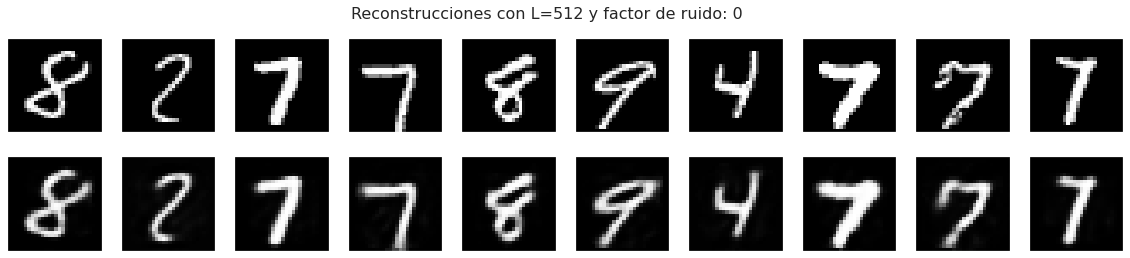
\includegraphics[width=13cm,keepaspectratio]{./graficos/test_0.png}
  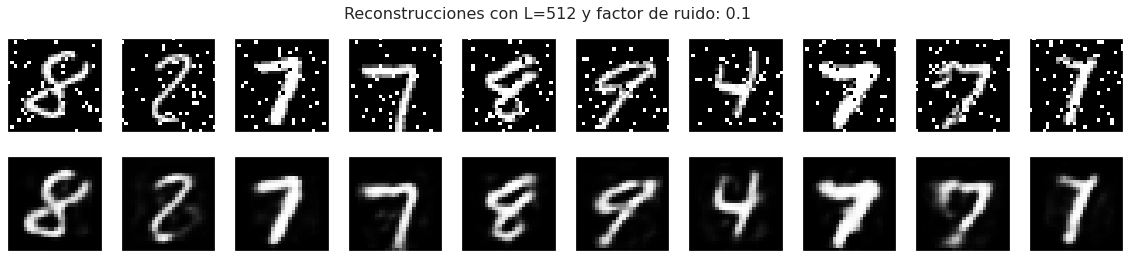
\includegraphics[width=13cm,keepaspectratio]{./graficos/test_0_1.png}
  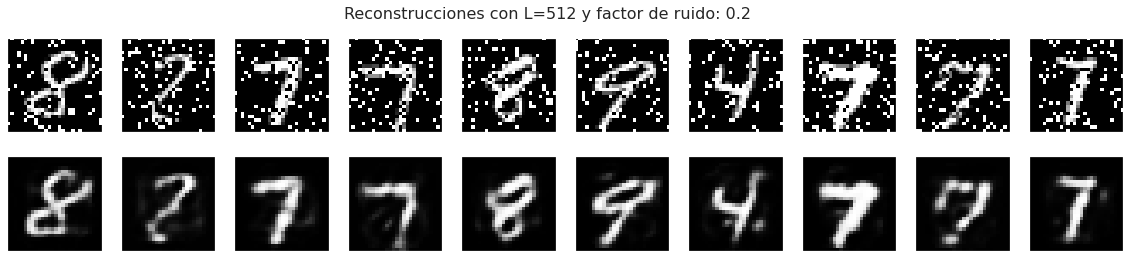
\includegraphics[width=13cm,keepaspectratio]{./graficos/test_0_2.png}
  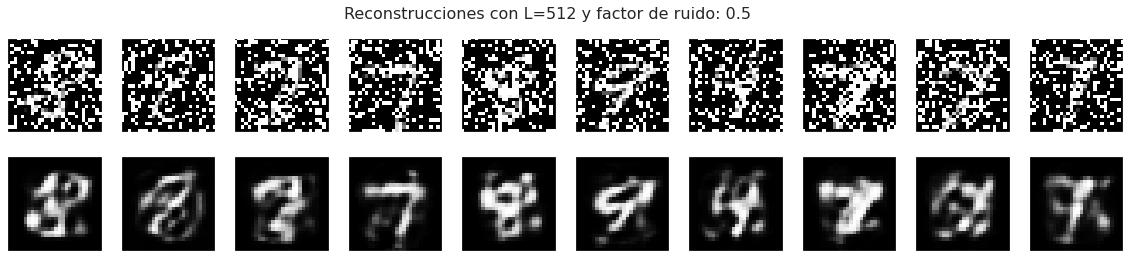
\includegraphics[width=13cm,keepaspectratio]{./graficos/test_0_5.png}
  \caption{Test del modelo para $L=64$ con distintos factores de ruido.}\label{fig:test}
\end{figure}

En la figura \ref{fig:test} podemos observar que a medida que el factor de ruido crece, el modelo tiene más problemas para reconstruir la imágen. Al probar con un factor de ruido $0.5$, apenas podemos distinguir los dígitos reconstruidos. Sin embargo, para factores razonables, nuestro modelo provee una reconstrucción fiel del dígito. 

\section{Búsqueda y análisis}

En esta sección vamos a variar el valor del parámetro $L$, que corresponde a la cantidad de neuronas de la capa oculta, en los siguientes valores: $L \in [128, 256, 512]$. Para estos casos, vamos a comparar las curvas dadas por la pérdida y la accuracy del modelo.

\pagebreak

\begin{figure}[ht]
  \centering
  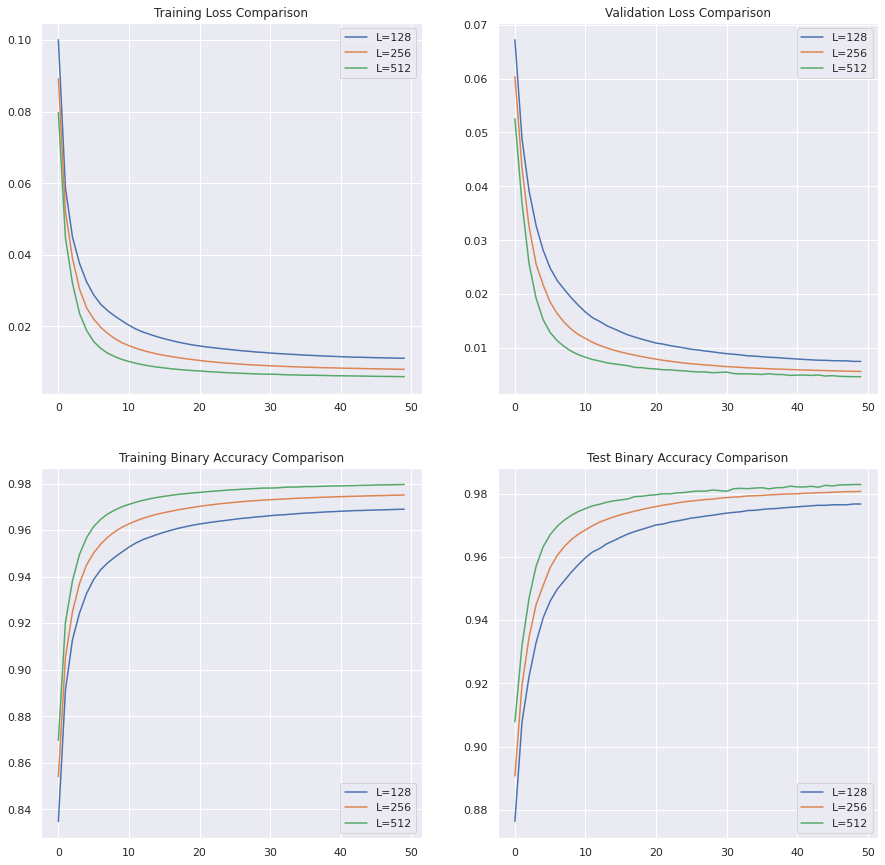
\includegraphics[width=15cm,keepaspectratio]{./graficos/metrics_comparison.png}
  \caption{Comparación de las métricas de entrenamiento y test con disintos valores para $L$}\label{fig:metrics_comparison}
\end{figure}

Como podemos observar en la figura \ref{fig:metrics_comparison}, mientras más neuronas tiene nuestra capa oculta, más rápidamente convergen las métricas hacia algún valor. Sin embargo, los valores finales de pérdida y accuracy no parecen tener una diferencia significativa.

\section{Conclusión}

Al comparar distintos modelos, vimos que mientras más neuronas tenemos, más rápido aprende nuestro modelo y obtenemos mejores métricas. Esto se debe a que la compresión de las imágenes guarda más datos mientras más neuronas ocultas tenemos y esto permite que nuestro modelo reconstruya mejor la imágen. Sin embargo, a pesar de tener mejores resultados, el tener más neuronas en nuestra capa oculta influye directamente en el tiempo de cómputo de nuestro modelo y en su peso en memoria. Además, al aumentar la cantidad de neuronas de la capa oculta, también corremos más riesgo de sobreajuste (overfitting), ya que un modelo muy complejo no generaliza para disminuir la pérdida, si no que generaliza únicamente los datos del entrenamiento.


\end{document}
